% DOCUMENT FORMATING
\documentclass[12pt]{article}
\usepackage[margin=1in]{geometry}

% PACKAGES
\usepackage{amsmath} % For extended formatting
\usepackage{amssymb} % For math symbols
\usepackage{amsthm} % For proof environment
\usepackage{array} % For tables
\usepackage{enumerate} % For lists
\usepackage{extramarks} % For headers and footers
\usepackage{fancyhdr} % For custom headers
\usepackage{graphicx} % For inserting images
\usepackage{multicol} % For multiple columns
\usepackage{verbatim} % For displaying code
\usepackage{tkz-euclide}
\usepackage{pgfplots}
\usepackage{mathtools}


% SET UP HEADER AND FOOTER
\pagestyle{fancy}
\lhead{\MyCourse} % Top left header
%\chead{\MyTopicTitle} % Top center header
\rhead{\MyAssignment} % Top right header
%\lfoot{\MyCampus} % Bottom left footer
\cfoot{} % Bottom center footer
%\rfoot{\MySemester} % Bottom right footer
\renewcommand\headrulewidth{0.4pt} % Size of the header rule
\renewcommand\footrulewidth{0.4pt} % Size of the footer rule




% ----------
% TITLES AND NAMES 
% ----------

\newcommand{\MyCourse}{Math 241}
\newcommand{\MyAssignment}{Worksheet 9}
%\newcommand{\MySemester}{Spring 2020}
%\newcommand{\MyCampus}{University of Hawaii at Manoa}

% ----------
% BEGIN DOCUMENT
% ----------


\begin{document}
\begin{enumerate}
    \item Let $f''(x) = 12x^2 + 6x + 8$.
    \begin{enumerate}
        \item Find $f'(x)$ and $f(x)$.
        \vspace{2in}
        \item Suppose that $f'(1) = 2$ and $f(0) = 6$. Find the particular $f(x)$.
    \end{enumerate}
    \pagebreak
    \item Let $f''(x) = 8x^3 + 2x - 4$.
    \begin{enumerate}
        \item Find $f'(x)$ and $f(x)$.
        \vspace{2in}
        \item Suppose $f(-1) = 3$ and $f(2) = -4$. Find the particular $f(x)$.
    \end{enumerate}

    \pagebreak

    \item Below is the graph of the function $f(x) = -x^2+4$.
    \begin{center}
        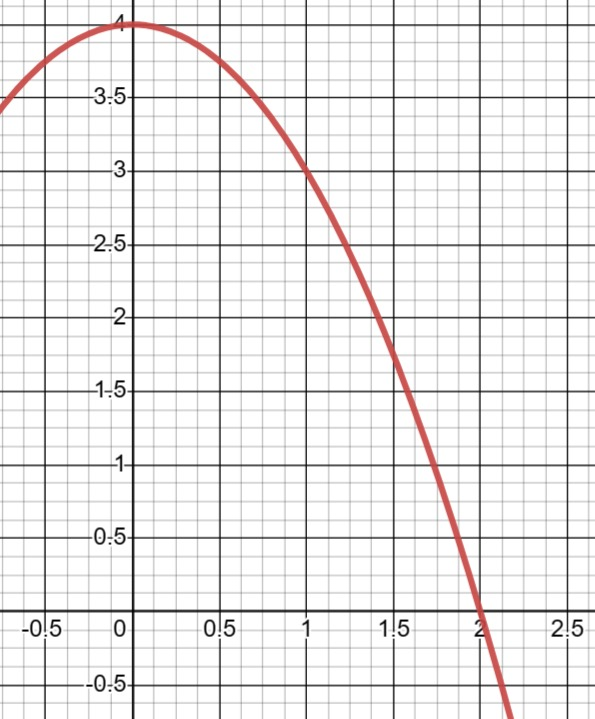
\includegraphics[scale=0.4]{Images/S23 M215 PMT3 pic1.jpeg}
    \end{center}

    \begin{enumerate}
        \item Using $n=4$ rectangles with equal bases, approximate the area under the curve of $f(x) = -x^2+4$ over the interval $[0,2]$ using a left end point approximation.
        \vspace{1.5in}
    
        \item On the graph, draw the four rectangles.
        \item Is your approximation in (a) an overestimate or underestimate of $\int_0^2 f(x)\,dx$? Justify why.
    \end{enumerate}

    \pagebreak

    
    \item Find the derivative $\frac{dy}{dx}$ of the following.
    \begin{enumerate}
        \item $y=\displaystyle\int_0^{x^2} \sin(\sqrt{t+7})\, dt.$
        \vfill
        \item $y=\displaystyle\int^0_{\sin(x^2)} \cos\left(\dfrac{t}{t^2+1}\right)\, dt$
        \vfill
        \item $y=\displaystyle\int_{x^2}^{x^3} \sqrt{t^{3/2}+4}\, dt$
        \vfill
    \end{enumerate}
\end{enumerate}
\end{document}